
\section{Improving Semantics}\label{sec:mapping}

More than improving the current infrastructure for storing and
accessing CPDOC data, we would like to exploit the semantic
possibilities of such rich source of knowledge. One of the ways to do
that is to embed knowledge from other sources by creating links within
the available data. Since much of the data is related to people and
resources with historical relevance, or historical events, some
available ontologies and vocabularies can be used in this task.

The personal nature of the data allows us to use projects that are
already well developed for describing relationships and bonds between
people, such as FOAF~\cite{foaf} (Friend of a Friend) -- a vocabulary
which uses RDF to describe relationships between people and other
people or things. FOAF permits intelligent agents to make sense of the
thousands of connections people have with each other, their belongings
and historical positions during life. This improves accessbility and
generates more knowledge from the available data.

The analysis of structured data can automatically extract connections
and, ultimately, knowledge. A good example is the use of
PROV~\cite{prov}, which provides a vocabulary to interchange
provenance information. This is interesting to gather information of
data that can be structurally hidden in tables or tuples.  
% For instance [EXAMPLE].

The RDF graph model enables also the merging of data content
naturally. The DBpedia project, for instance, allows users to query
relationships and properties associated with Wikipedia resources, and
users can link other datasets to the DBpedia dataset in order to
create a big and linked knowledge knowledge base.
% The DBpedia project, for instance, provide URIs~\footnote{Uniform
% resource identifier,
% \url{https://en.wikipedia.org/wiki/Uniform_resource_identifier}.}
% which enable the connection of these resources with different
% sources of data in order to create a big and linked knowledge
% database.
CPDOC can use DBpedia to link their data to already available
resources in DBpedia making their own data available to a bigger
audience.

In the same direction, we aim to use of lexical databases, such as the
WordNet~\cite{wordnet} and its Brazilian version
OpenWordnet-PT~\cite{wordnet-br}, to make natural language processing
of DHBB entries. For instance, named entities recognizition and other
NLP tasks can create automatically connections that improve
dramatically the usability of the content.
% The Brazilian OpenWordnet-PT provides a lexical resource for
% Portuguese complete mapped to the original english WordNet.
Other resources like YAGO~\cite{yago} and BabelNet~\cite{babelnet}
links Wikipedia to WordNet. The result is an ``encyclopedic
dictionary'' that provides concepts and named entities lexicalized in
many languages and connected with large amounts of semantic
relations. Finally, the SUMO Ontology~\cite{sumo} could also be used
to provide a complete formal definition of terms linked to
WordNet. All of these lexical resources and ontologies will be further
explored when we start the natural language processing of DHBB
entries.

% Much of the effort proposed is related to integrating the data
% available to other sources of knowledge, improving both
% accessibility and usability of the data CPDOC holds. To do so, it is
% imperative to migrate the current CPDOC database model to a open,
% shared and modern one, aligned with semantic web directives,
% ontologies and vocabularies. This improvement is highlighted is what
% we called the refinement of the RDF model when we described
% Figure~\ref{fig:dia-1}.  It what follows, let us give an example of
% the proposal refinement considering a fragment of the original CPDOC
% relational model.

\begin{figure}[htbp]
  \centering
  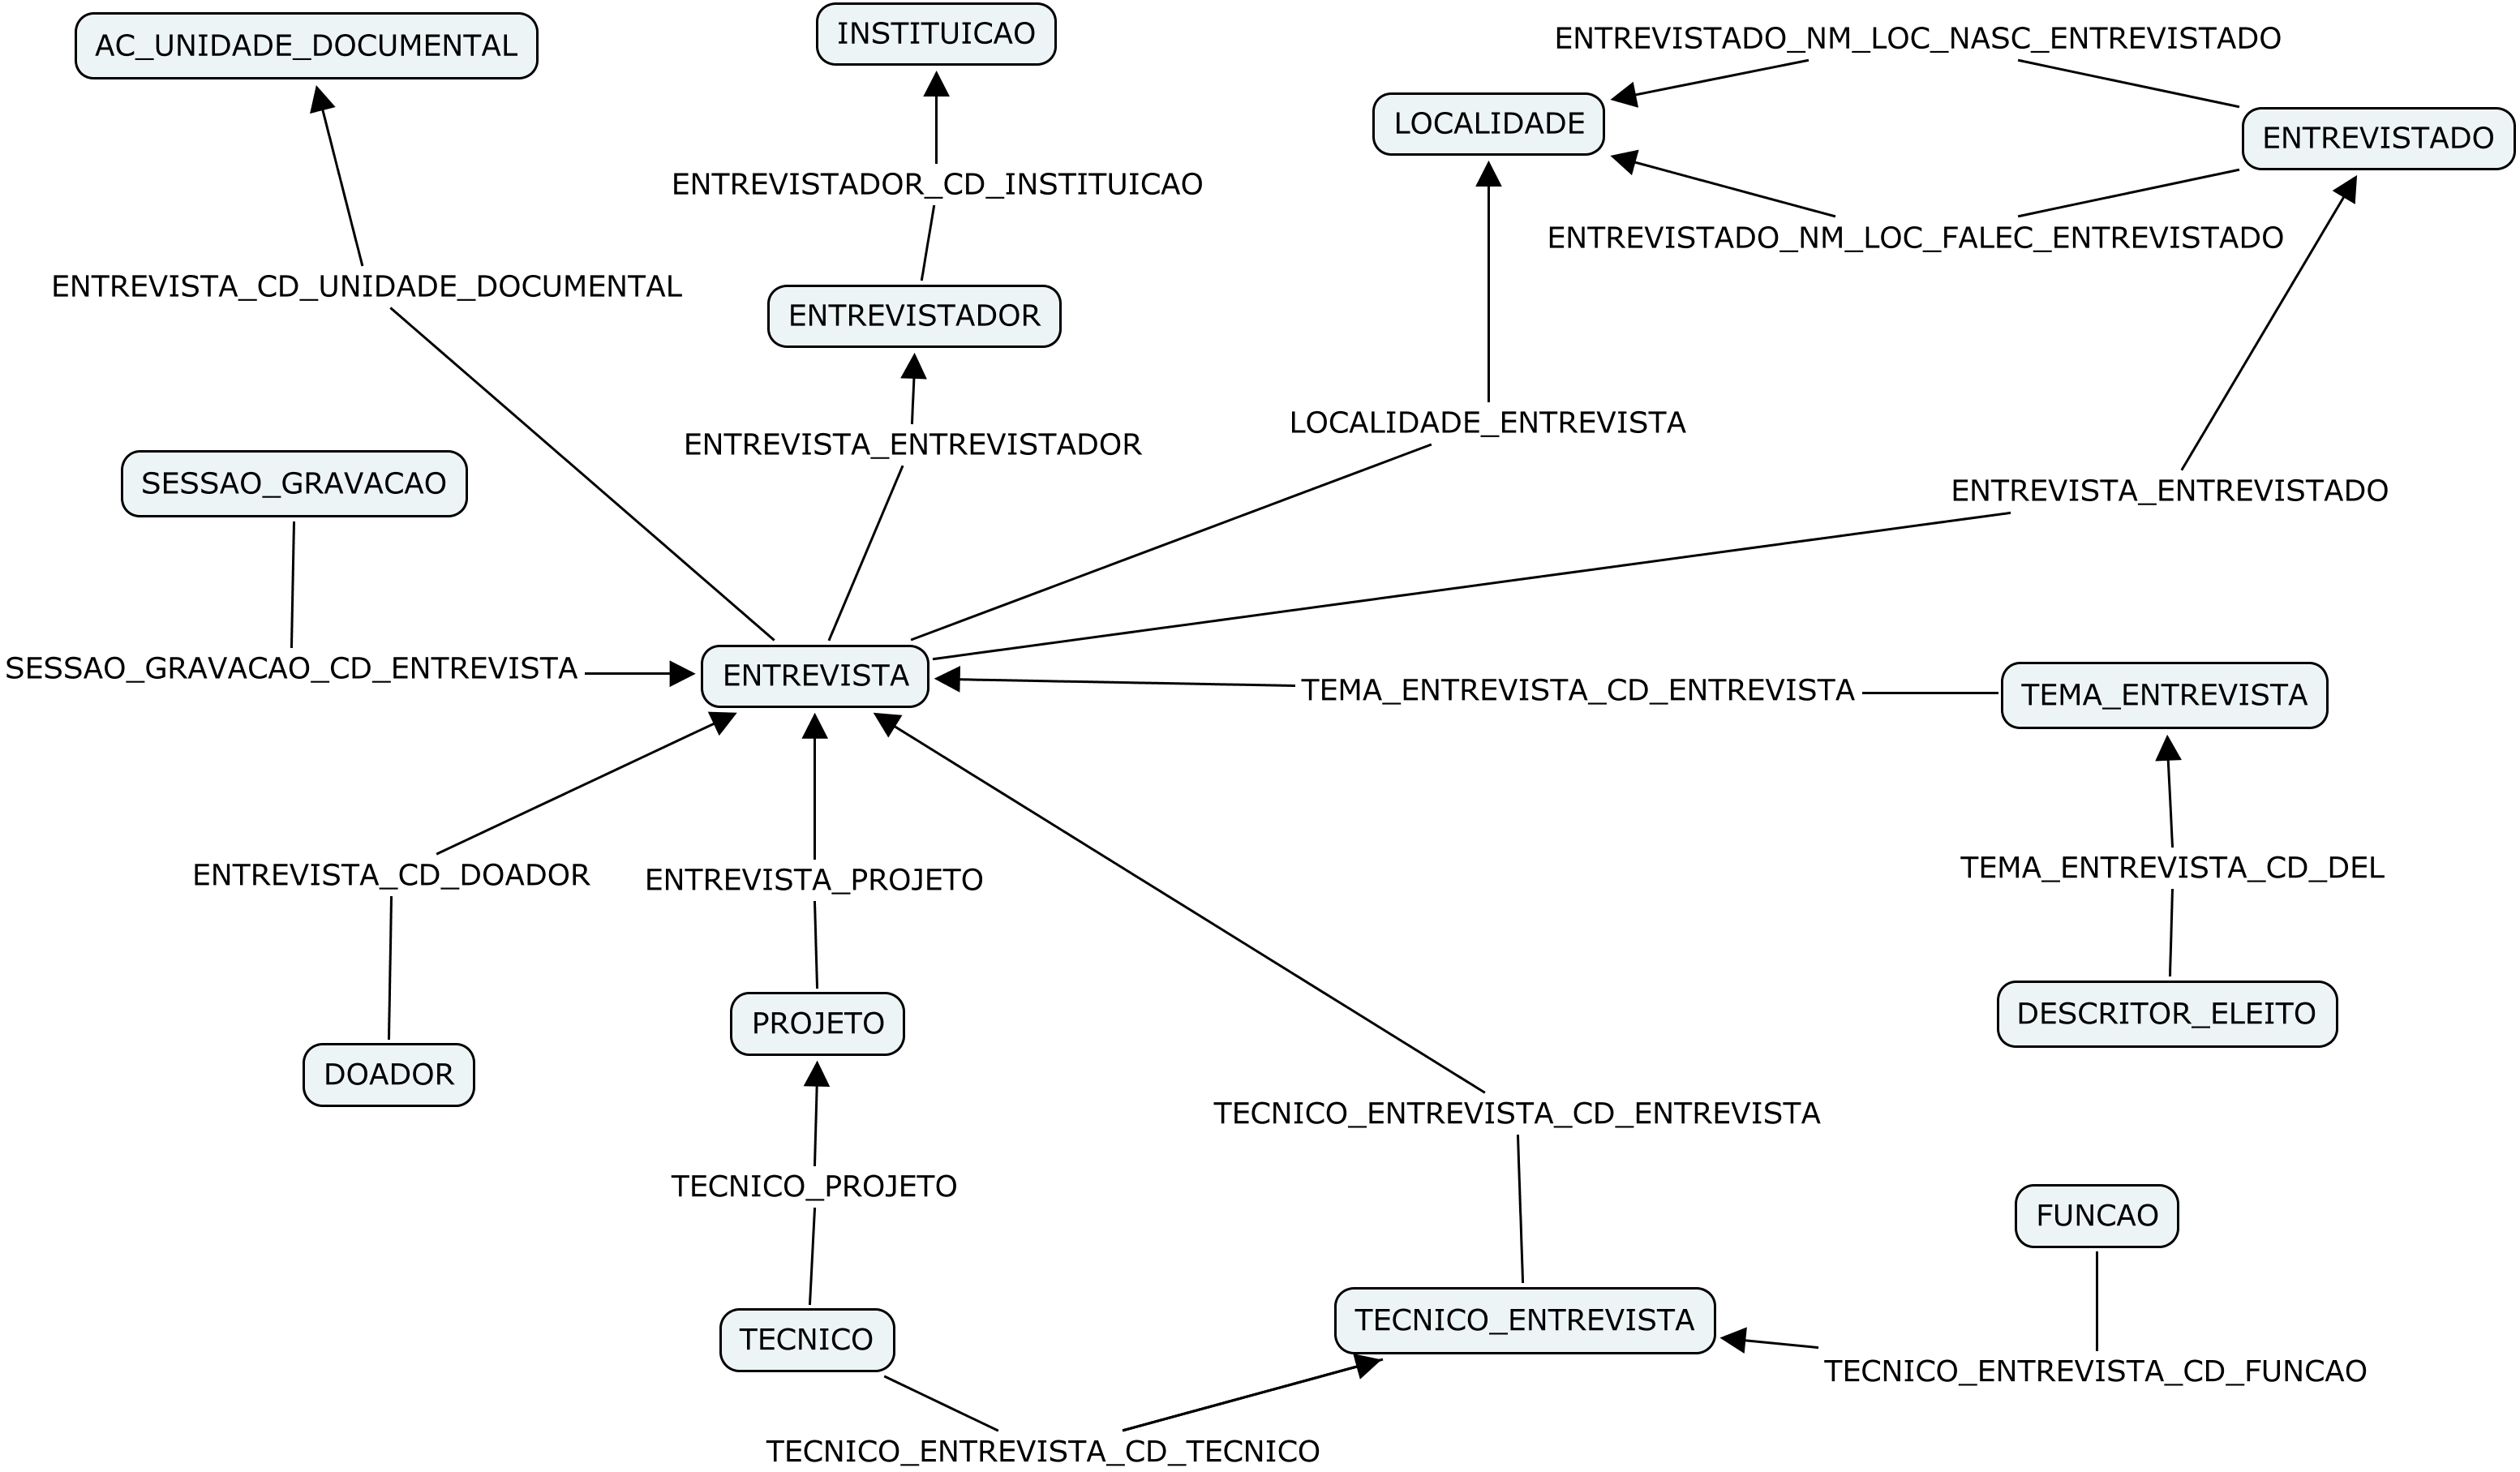
\includegraphics[width=.8\textwidth]{pho.png}
  \caption{PHO first RDF model}\label{fig:pho}
\end{figure}

% What is important to note in the model presented in
% Figure~\ref{fig:pho} is that besides simple translations from
% relational to graph model, D2RQ was not able to automatic improve
% much further the model. Let us highlight some cases. D2RQ was able
% to correctly translate relations N:M in the relational model, such
% as \texttt{entrevista\_entrevistador} (originally a table in the
% relational model) to a property that connect directly instances of
% \texttt{entrevista} (Interview) with instances of
% \texttt{entrevistador} (Interviewer). Nevertheless, the N:M relation
% between \texttt{entrevista} and \texttt{tecnico} (technician) was
% kept as a a intermediary class called \texttt{tecnico\_entrevista}
% because of the existence of an aditional information in this N:M
% relation, the role (\texttt{funcao} class) of the technician in the
% interview. More on roles, the relational model also expose some
% inconsistences. Althought connection of the technician and the
% interview is parameterize by its role, the donator, interviewer and
% the interviewee of the interview are modelled each one by a specific
% table. The main problem with this model is that interviewee,
% interviewer, donator and technician are all people with share a lot
% of common properties like name, address and so on. These problems
% are all result of a ``ad hoc'' modeling process. The model, as is,
% only makes sense for CPDDOC team and it could hardly be useful
% outside CPDOC.


Figure~\ref{fig:pho} shows a fragment of the current RDF model
produced by D2RQ, in step (1) of Figure~\ref{fig:dia-1}, using the
original CPDOC database relational model. This fragment exposes only
the PHO classes (derived from the tables) and some properties (derived
from the foreign keys). Classes are written inside the boxes and the
names in arrows that connect the boxes are the properties that connect
instances of the classes.

In the model presented in Figure~\ref{fig:pho} it is possible to see
that D2RQ was not able to automaticly improve much further the
model. D2RQ was able to correctly translate relations N:M in the
relational model, such as \texttt{entrevista\_entrevistador}
(originally a table in the relational model) to a property that
connect directly instances of \texttt{entrevista} (Interview) with
instances of \texttt{entrevistador} (Interviewer). Nevertheless, the
N:M relation between \texttt{entrevista} and \texttt{tecnico}
(technician) was kept as a a intermediary class called
\texttt{tecnico\_entrevista} because of the existence of an aditional
information in this N:M relation, the role (\texttt{funcao} class) of
the technician in the interview. The relational model also seems to
have some inconsistences. Although the connection of technician and
interview is parameterized by different roles, the donator,
interviewer and interviewed of an interview are modelled each one in a
specific table. In this case interviewed, interviewer, donator and
technician are all people that share a lot of common properties like
name, address, etc, and could be modeled as people. These problems are
all result of a ``ad hoc'' modeling process. The model, as is, only
makes sense for CPDDOC team and it could hardly be useful outside
CPDOC.

\begin{figure}[htbp]
  \centering
  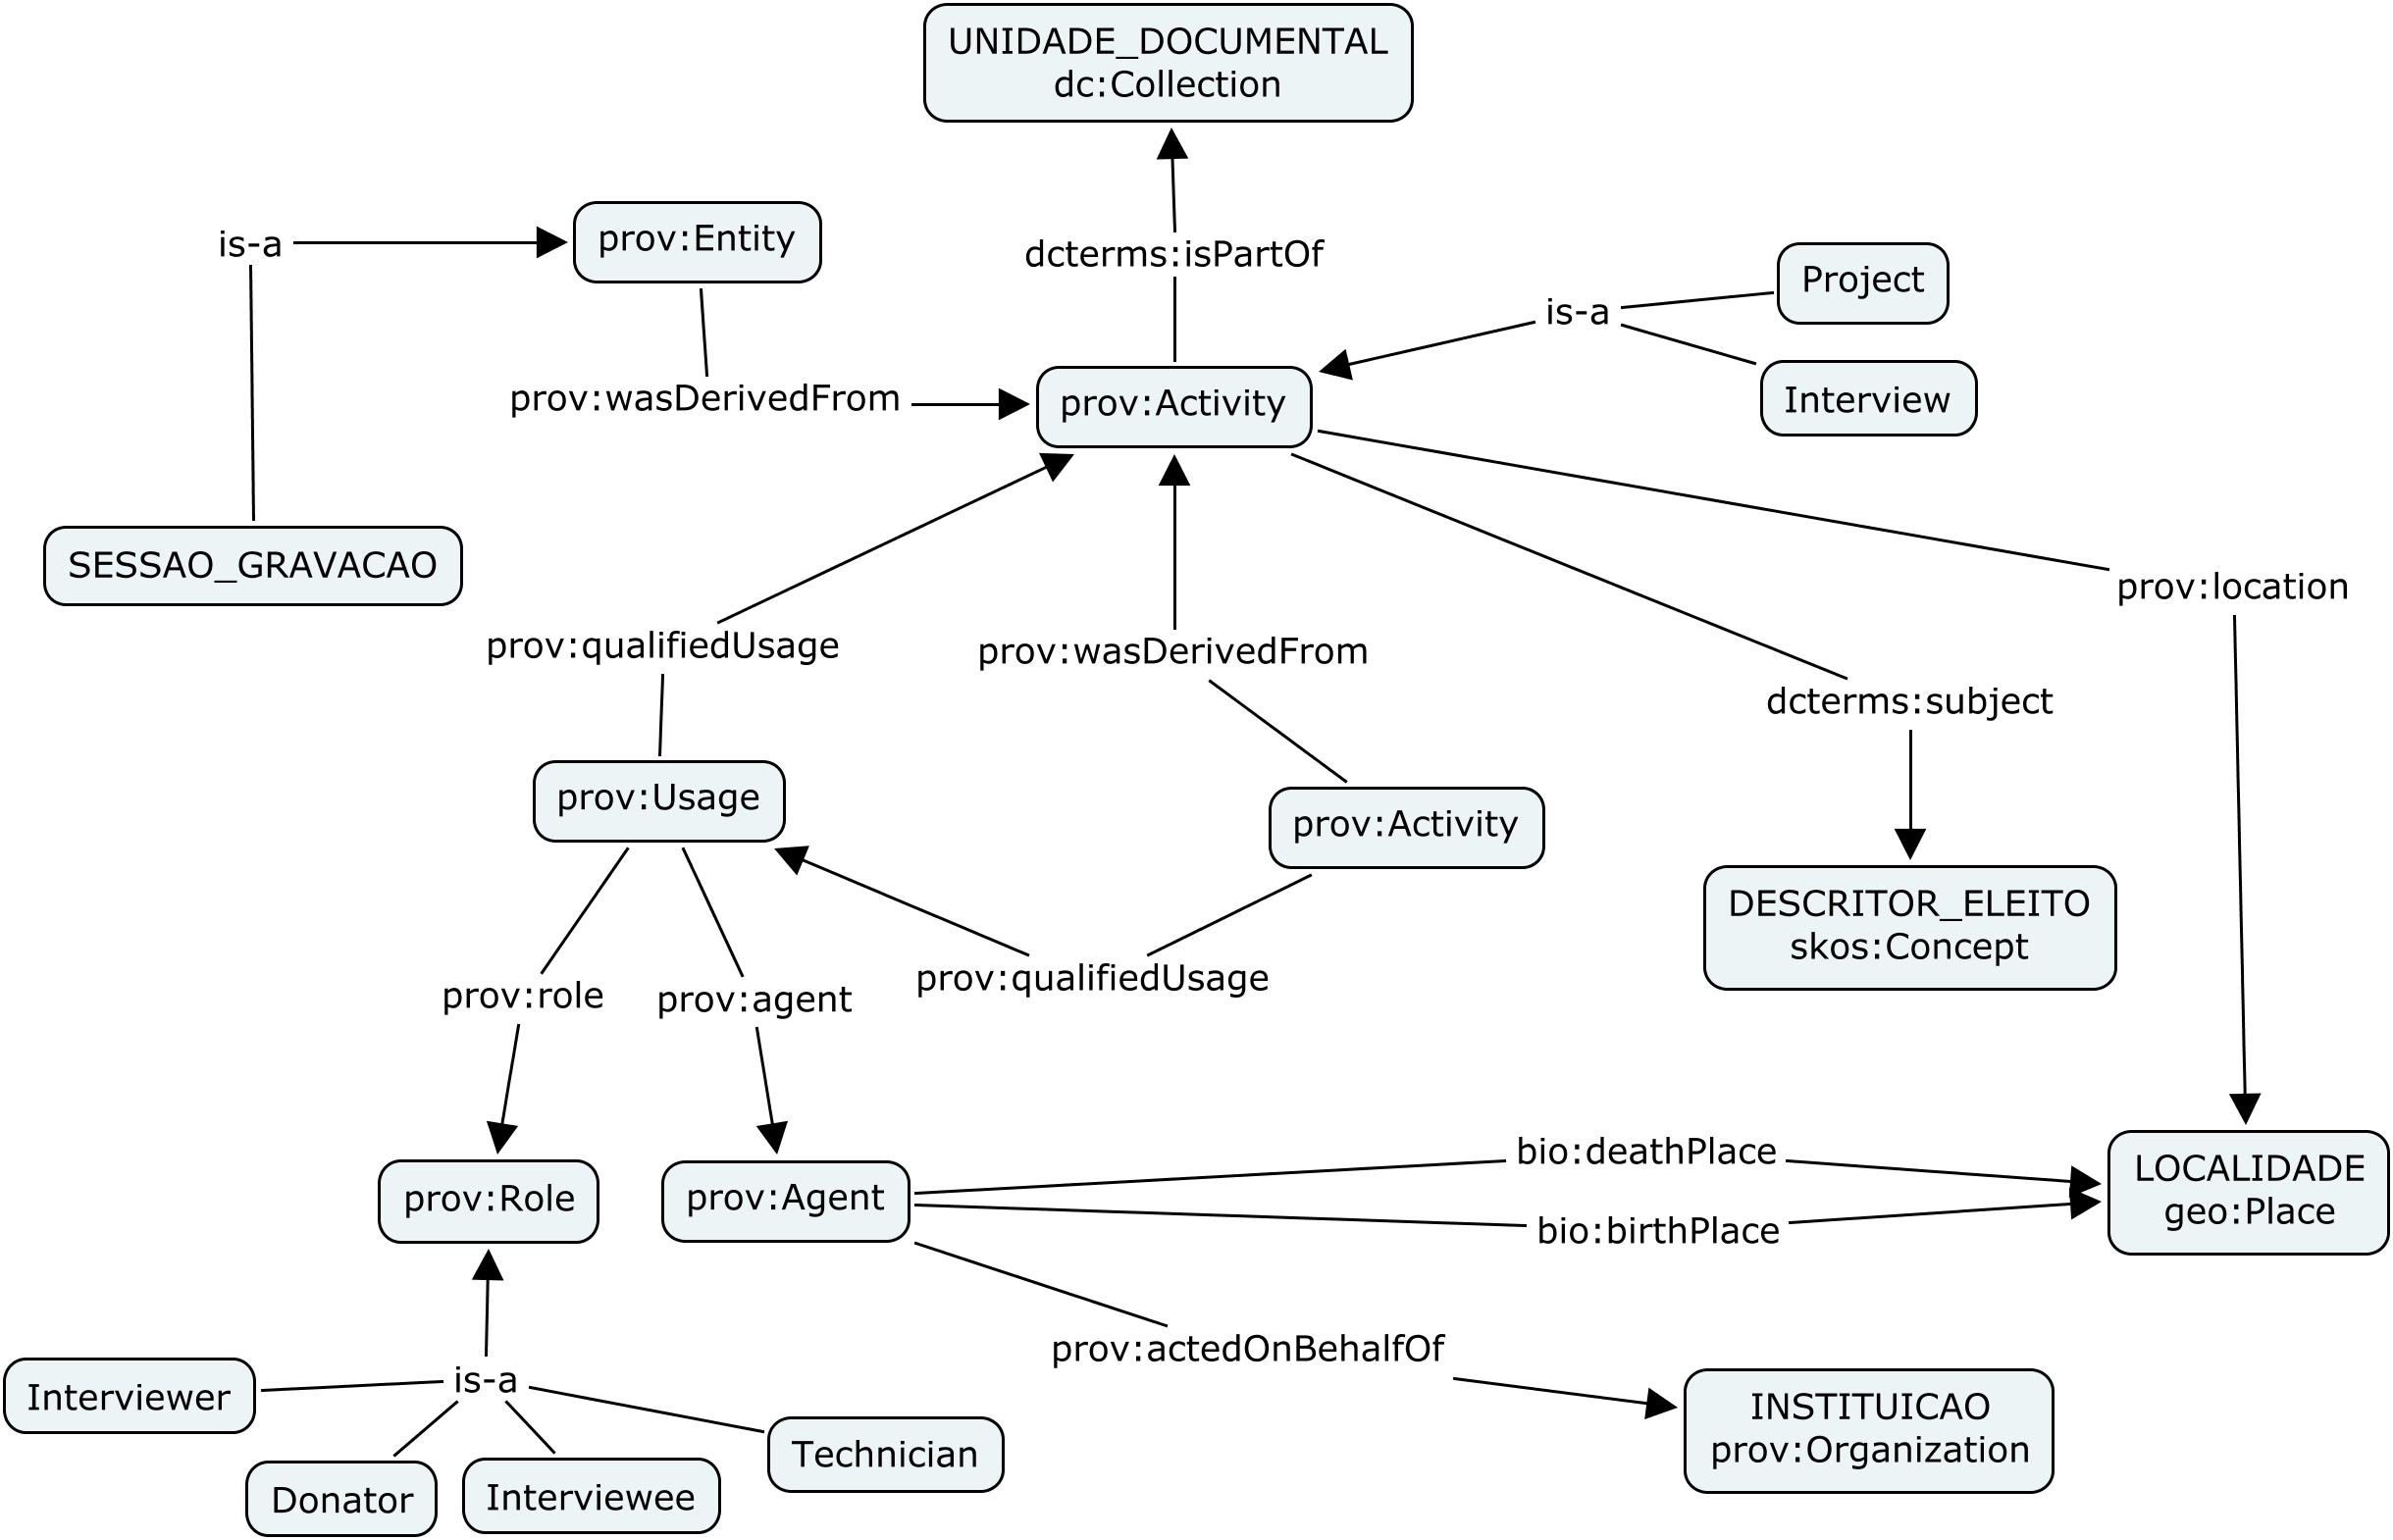
\includegraphics[width=.8\textwidth]{pho-new.png}
  \caption{PHO revised RDF model}\label{fig:pho-new}
\end{figure}

Figure~\ref{fig:pho-new} shows how PHO model will be refined. The new
model uses standard vocabularies and ontologies, making the whole
model much more understandable and interoperable. In the
Figure~\ref{fig:pho-new}, \texttt{prov:Activity} was duplicated just
to better presentation. The prefixes in the names indicate the
vocabularies and ontologies used: \texttt{prov}, \texttt{skos},
\texttt{dcterms}, \texttt{dc}, \texttt{geo}, and \texttt{bio}. We also
developed a CPDOC ontology that declares its own classes and specify
ontologies links like the one that says that an \texttt{foaf:Agent} is
a \texttt{prov:Agent}. Some classes will be subclasses of standard
classes (e.g. \texttt{Interview}), some will be replaced by standard
classes (e.g. \texttt{LOCALIDADE}). 

%%% Local Variables: 
%%% mode: latex
%%% TeX-master: "article"
%%% End: 
